
%%%%%%%%%%%%%%%%%%%%%%%%%%%%%%%%%%%%%%%%%%%%%%%%%%%%%%%%%%%%%%%%%%%%%%%%%%%%%%%
%
% witseiepaper-2005.tex
%
%                       Ken Nixon (12 October 2005)
%
%                       Sample Paper for ELEN417/455 2005
%
%%%%%%%%%%%%%%%%%%%%%%%%%%%%%%%%%%%%%%%%%%%%%%%%%%%%%%%%%%%%%%%%%%%%%%%%%%%%%%%%

\documentclass[10pt,twocolumn]{witseiepaper}

%
% All KJN's macros and goodies (some shameless borrowing from SPL)
\usepackage{KJN}
\usepackage{hyperref}
\usepackage{xcolor}

%
% PDF Info
%
\ifpdf
\pdfinfo{
/Title (INSTRUCTIONS AND STYLE GUIDELINES FOR THE PREPARATION OF FINAL YEAR LABORATORY PROJECT PAPERS : 2005 VERSION)
/Author (Ken J Nixon)
/CreationDate (D:200309251200)
/ModDate (D:200510121530)
/Subject (ELEN417/455 Paper Format, 2005)
/Keywords (ELEN417, ELEN455, paper, instructions, style guidelines, laboratory project)
}
\fi

%%%%%%%%%%%%%%%%%%%%%%%%%%%%%%%%%%%%%%%%%%%%%%%%%%%%%%%%%%%%%%%%%%%%%%%%%%%%%%%
\begin{document}


\title{INSTRUCTIONS AND STYLE GUIDELINES FOR THE PREPARATION OF FINAL YEAR LABORATORY PROJECT PAPERS : 2005 VERSION}

\author{Elias Sepuru (1386807)
\thanks{School of Electrical \& Information Engineering, University of the
Witwatersrand, Private Bag 3, 2050, Johannesburg, South Africa}
}


%%%%%%%%%%%%%%%%%%%%%%%%%%%%%%%%%%%%%%%%%%%%%%%%%%%%%%%%%%%%%%%%%%%%%%%%%%%%%%%
%
\abstract{The purpose of this document is to provide an easy-to-use
template/style sheet to enable authors to prepare papers in the correct format
and style for the final year laboratory project. This document may be
downloaded from the School of Electrical and Information Engineering web site
and can be used as a template. To ensure conformity of appearance it is
essential that these instructions are followed. The abstract should be limited
to 50-200 words, which should concisely summarise the paper.}

\keywords{Four to six key words in alphabetical order, separated by commas.}


\maketitle
\thispagestyle{empty}\pagestyle{empty}


%%%%%%%%%%%%%%%%%%%%%%%%%%%%%%%%%%%%%%%%%%%%%%%%%%%%%%%%%%%%%%%%%%%%%%%%%%%%%%%
%
\section{INTRODUCTION}
\label{intro}
As it stands, one of the most important, cost-effective and widely used techniques for one to get screened for cardiovascular diseases (CVDs) is through cardiac auscultation by a clinical physician \cite{28_gavrovska2017identification, 32_montinari2019first}. For rural populations, screening for CVDs hardly occurs due to lack of clinical physicians and health care avoidance \cite{33,34}. World Health Organisation (WHO) reports CVDs as the leading cause of deaths globally, with an estimated 31\% of the deaths in 2016 caused by CVDs \cite{WHO}. Methods to detect early signs of CVDs could prove to be very helpful in lowering the mortality rate due to CVDs, especially in disadvantaged communities \cite{34}.

This paper presents a project, that aims create an application using machine learning techniques. The application will enable first level screening of CVDs for personal use by individuals on their smartphones and will aid clinical physicians with cardiac auscultation. To train the machine learning (ML) models, heartbeat sounds, in a form of a Phonocardiogram (PCG) signal, from two sources are used. The sources are a smartphone and a digital stethoscope. Prior training, the PCG signals are segmented and used to generate features to feed the ML models. A total of 24 features, including non-time-domain features, are extracted. The ML models (ANN, SVM \& XGB) trained on these features are then compared in their ability to diagnose CVDs.

%%%%%%%%%%%%%%%%%%%%%%%%%%%%%%%%%%%%%%%%%%%%%%%%%%%%%%%%%%%%%%%%%%%%%%%%%%%%%%%%%%%%%%%%%%%%%%%%%%%%%%%%%%%%%%%%%%%%%%%%%%%%%%%%%%%%

\section{BACKGROUND}
\label{back}
Through cardiac auscultation clinical physicians are able to tell whether an individual has CVDs or not. They use the heart's lub (S1) and dub (S2) sounds to help them identify irregularities in ones heartbeat sounds. S1 and S2 are known as the fundamental heart sounds (FHSs) \cite{54}. The intervals between S1-S2 and S2-S1 are known as the systolic and diastolic periods respectively. For a relaxed heartbeat the diastolic period is larger than the systolic period \cite{orient2010sapira}. In a normal heartbeat sound, S1 is followed by S2 in a continuous cycle.

Abnormalities occur when there are irregularities in the cycle of S1 and S2, these irregularities are what makes CVDs. 

As mentioned in section \ref{intro} , the heartbeat audio data is from two sources, a smartphone (Dataset A) and a digital stethoscope (Dataset B). Dataset A has four classes: Normal, Murmur, Extra Heart Sound (HS) and Artifact. Dataset B has has three classes: Normal, Murmur and Extrasystole. 

Murmurs are produced when there is a turbulent blood flow between either systolic or diastolic periods \cite{35}. The turbulence often cause a "whooshing" sound in between S1 and S2. Extra HS are produced when there is either an extra S2 or S1 after either S2 or S1 has occurred. This repeats regularly throughout the entire heart cycle in this manner: S1-S2-S2-S1 or S1-S1-S2-S1-S1. Extrasystole occur in a similar manner as Extra HS, but they do not occur regularly \cite{bentley}. See Appendix \ref{HS}, for a clearer explanation of the distinctions between the different classes and an explanation of the \hyperref[sec:arti]{Artifact} class.

\subsection{PROJECT FRAMEWORK}
\subsubsection{Project Specifications and Requirements}
\label{sec:req}
\textcolor{white}{Ke a leboga Ntate}\\
The ultimate aim of the project is create an application using ML techniques that will aid patients and clinical physicians in early detection of CVDs. The application is to accept raw audio data as input and return diagnosis results as an output.

This will be carried out using data from Dataset A and Dataset B. Dataset A is recorded by the general public using the iStethoscope Pro app on an iPhone, whilst Dataset B is recorded in a more professional manner by clinical physicians using a digital stethoscope. They both differ by two categories as mentioned in the opening paragraphs of section \ref{back} and both have excessive background noise as they are recorded in real-life settings. 

Due to the excessive background noise, it is required that processing techniques capable of denoising the audio data be implemented before segmentation can occur. Following denoising, a method to locate S1 and S2 HSs as well as a method to segment the Normal PCGs from both datasets is required. After successful segmentation, it is required that features be generated from the results of segmenting the PCG signals. Lastly, it is required that ML models be built and trained using the generated features. 

\subsubsection{Assumptions}
\textcolor{white}{Ke a leboga Jeso}\\
The project is to be conducted under the following assumptions:
\begin{itemize}
    \item The audio data range will be 30 seconds or less.
    \item Dataset A has only four classes ( Normal, Murmur, Extra HS and Artifact). Dataset B has only three classes ( Normal, Murmur \& Extrasystole)
    \item Both datasets have integrity and are correctly labelled.
\end{itemize}

\subsubsection{Constraints}
\label{sec:constraints}
\textcolor{white}{O re swarele...}\\
The following are the constraints imposed on the project:
\begin{itemize}
    \item Segmentation is based only on S1 and S2 sounds.
    \item Only the dataset from reference \cite{bentley} is to be used due to ethics clearance attached in Appendix \ref{ethics}.
    \item Only the Normal audio data will be used as a basis for the location of S1 and S2 and as a basis for segmentation.
    \item The audio data is only available in \texttt{.wav} and \texttt{.aif} formats.
\end{itemize}

\subsubsection{Success Criteria}
\textcolor{white}{O re swarele...}\\
The project is deemed successful if all requirements in section \ref{sec:req} have been met, whilst adhering to the set constraints in section \ref{sec:constraints}. Existing solutions
have an accuracy of up to 77\% for classifying Normals of Dataset B and an accuracy of up to 46\%
for Normals of Dataset A. With that said an accuracy of 77\% or higher in classifying Normals of Dataset B and
an accuracy of 46\% or higher in classifying Normals of Dataset A would be highly desirable.

\subsection{RELATED WORK}
Despite the medical significance of using ML techniques to detect for heart sounds (HSs) anomalies, this application of ML is relatively unexplored \cite{bentley}. There also exist a few studies that have done work in classifying various heartbeat sounds using these techniques \cite{26}. Of a few that exist majority of them use PCG signals \cite{53,51,36,37} whilst others use Electrocardiograms (ECG) signals \cite{4,5}. 

Before classification can occur, the HSs have to first be preprocessed and segmented. Liang \textit{et al} \cite{6} dominate in a lot of work \cite{11,19,15,50} with their method of preprocessing and segmenting HSs. Some of their method are adopted from Groch \textit{et al} \cite{2}. 

The features extracted from segmentation of HSs are usually time-domain based. Strunic \textit{et al} \cite{3} detects and classifies simulated murmurs \& normal HSs using similar preprocessing and segmentation techniques to \cite{6}. He trains a 3 hidden layer, 25 input and 1 output Artificial Neural Network (ANN) with simulated HSs. The ANN classifier achieves an accuracy of $85\pm7.4\%$ when tested with simulated HSs, however when tested with real-life HSs the accuracy drops to $48.7\pm12.7\%$. Unlike Strunic, Gomes \textit{et al} \cite{gomes2012classifying} train their ML models with real-life HSs having background noise. They extract time-domain features as well, using the standard deviation and mean of the systolic and diastolic periods intervals of the HSs. They achieve the highest accuracy of 72\% \& 70\% in classifying Normal HSs using the J48 Decision Tree and Multilayer Perceptron (MLP) respectively.

Instead of using time-domain features, Teo \textit{et al} \cite{17} segment HSs on the basis of S1, S2, systolic and diastolic periods. They take the Fast Fourier Transform (FFT) and Power Spectrum of each of the four segments and use them to train their Neural Network (NN).The NN achieves a total diagnosing accuracy of  77\%. 

Zhang \textit{et al} \cite{16} notice that using time or frequency domain features independently causes a loss in important pathological information. This leads to Tang \textit{et al} \cite{22} taking it one step further by combining a set of features from the time-domain, frequency-domain, cepstrum \& energy amongst others. With the same dataset as \cite{17}, they achieve an overall accuracy of 88\% using a Support Vector Machine (SVM) classifier.

%%%%%%%%%%%%%%%%%%%%%%%%%%%%%%%%%%%%%%%%%%%%%%%%%%%%%%%%%%%%%%%%%%%%%%%%%%%%%%%%%%%%%%%%%%%%%%%%%%%%%%%%%%%%%%%%%%%%%%%%%%%%%%%%%%%%
\section{CONCLUSION}

A conclusion may review the main points of the paper, but do not replicate the
abstract as the conclusion.


%%%%%%%%%%%%%%%%%%%%%%%%%%%%%%%%%%%%%%%%%%%%%%%%%%%%%%%%%%%%%%%%%%%%%%%%%%%%%%%


%%%%%%%%%%%%%%%%%%%%%%%%%%%%%%%%%%%%%%%%%%%%%%%%%%%%%%%%%%%%%%%%%%%%%%%%%%%%%%%
%
%\nocite{*}
\bibliographystyle{witseie}
\bibliography{sample}

%{\tiny \vfill \hfill \today \hspace{5mm} witseie-paper-2003.\TeX}



%%%%%%%%%%%%%%%%%%%%%%%%%%%%%%%%%%%%%%%%%%%%%%%%%%%%%%%%%%%%%%%%%%%%%%%%%%%%%%%%%%%%%%%%%%%%%%%%%%APPENDIX%%%%%%%%%%%%%%%%%%%%%%%%%%%%%%%%%%%%%%%%%%%%%%%%%%%%%%%%%%%%%%%%%%%%%%%%%%%%%%%%%%%%%%%%%%%%%%%%%%%%%%%%%%%%%%%%%%%%%%%%%%%%%%%%%%%%%%%%%%%%%%%%%%%%%%%%%%%%%%

\appendix
\section{Heart Sound Classes}
\label{HS}

\subsection*{The Normal Class}
The Normal class consists of normal, healthy and regular HS. A Normal HS has a clear \textit{"lub dub, lub dub"} or S1-S2-S1-S2. The illustration above shows the \textit{"lub, dub"} of a Normal HS over time \cite{bentley}.

\hspace{1cm}{\texttt{lub...dub......lub...dub.....}}

Figure \ref{fig:normal} illustrates a typical PCG of a Normal HS.
\begin{figure}[h!]
    \centering
    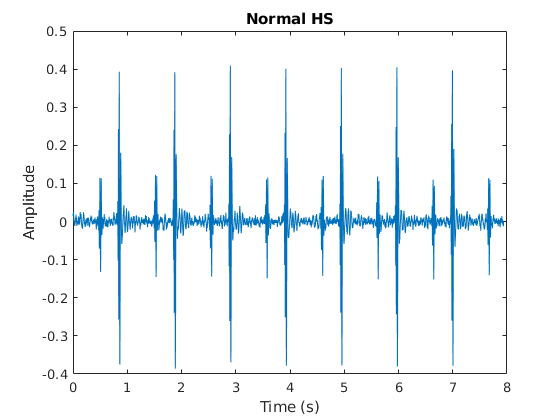
\includegraphics[scale = 0.45]{./normal.png}
    \caption{PCG of a Normal HS}
    \label{fig:normal}
\end{figure}{}

\subsection*{The Murmur Class}
The Murmur class consists of pathological HSs. Murmurs are produced when there is a turbulent blood flow between either systolic or diastolic periods \cite{35}. The turbulence often cause a "whooshing" sound in between S1 and S2 or in between S2 and S1. The illustration above shows the \textit{"lub, dub"} of a Murmur HS over time \cite{bentley}.

\hspace{1cm}{\texttt{lub..***..dub......lub..***..dub.....}}

\hspace{3.5cm} or 

\hspace{1cm}{\texttt{lub...dub...***...lub...dub..***...}}

Figure \ref{fig:murmur} illustrates a typical PCG of a Murmur HS.
\begin{figure}[h!]
    \centering
    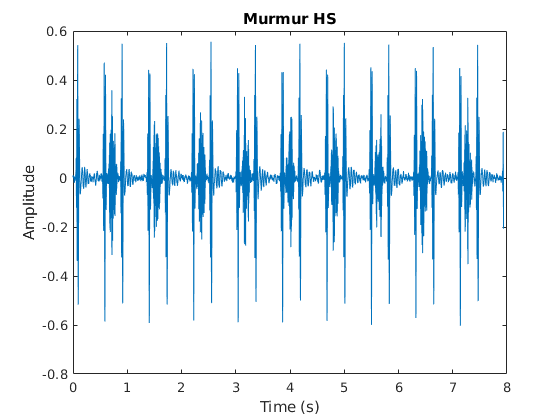
\includegraphics[scale = 0.45]{./murmur.png}
    \caption{PCG of a Murmur HS}
    \label{fig:murmur}
\end{figure}{}

From figure \ref{fig:murmur} it can clearly be seen that there are are extra disturbances in between S1 and S2 as compared to figure \ref{fig:normal}.

\subsection*{The Extra HS Class}
\label{sec:extra}
The Extra HS class does not necessarily consists of pathological HSs, however sometimes it could be a sign of a disease. Extra HS are produced when there is either an extra S2 or S1 after either S2 or S1 has occurred. This repeats regularly throughout the entire heart cycle in this manner S1-S2-S2-S1 or S1-S1-S2-S1-S1.
The illustration above shows the \textit{"lub, dub"} of a Extra HS over time \cite{bentley}.

\hspace{1cm}{\texttt{lub.lub...dub......lub.lub...dub.....}}

\hspace{3.5cm} or 

\hspace{1cm}{\texttt{lub...dub.dub.....lub...dub.dub.....}}

Figure \ref{fig:extra} illustrates a typical PCG of an Extra HS.
\begin{figure}[h!]
    \centering
    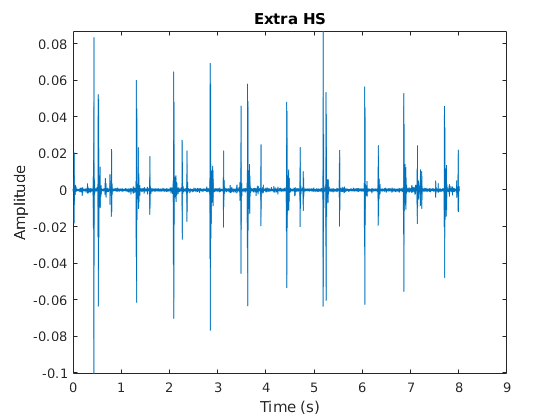
\includegraphics[scale = 0.45]{./extra.png}
    \caption{PCG of an Extra HS}
    \label{fig:extra}
\end{figure}{}

From figure \ref{fig:extra} it can clearly be seen that there are extra peak in between S1 and S2 as compared to figure \ref{fig:normal}.

\subsection*{The Extrasystole HS Class}
The Extrasystole class, similar to the \hyperref[sec:extra]{Extra HS} class, does not necessarily consists of pathological HSs, however sometimes it could be a sign of a disease. Extrasystole HSs occur in a similar manner as Extra HS, but they do not occur regularly. They are commonly identified by HSs that are out of place, with a HS either repeated or skipped. The illustration above shows the \textit{"lub, dub"} of a Extrasystole HS over time \cite{bentley}.

\hspace{0.5cm}{\texttt{lub....dub......lub.lub...dub.....lub....}}

\hspace{3.5cm} or 

\hspace{0.5cm}{\texttt{lub....dub.dub.....lub...dub......lub....}}

Figure \ref{fig:extrasys} illustrates a typical PCG of an Extrasystole HS.
\begin{figure}[h!]
    \centering
    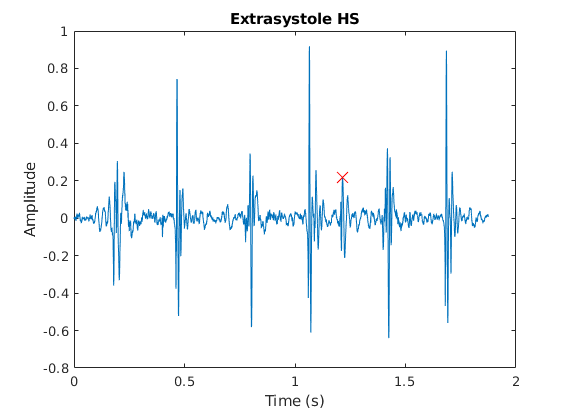
\includegraphics[scale = 0.45]{./extrasys.png}
    \caption{PCG of an Extrasystole HS}
    \label{fig:extrasys}
\end{figure}{}

From figure \ref{fig:extrasys} it can clearly be seen that there is a single extra peak in between S1 and S2, marked with a red cross, as compared to figure \ref{fig:normal} and figure \ref{fig:extra}.

\subsection*{The Artifact Class}
\label{sec:arti}
The Artifact class does not consist of any HSs. These are recordings of random sounds. The class is to help the developed models to differentiate between a HS and just pure noise \cite{bentley}.

Figure \ref{fig:arti} illustrates a typical of an Artifact.
\begin{figure}[h!]
    \centering
    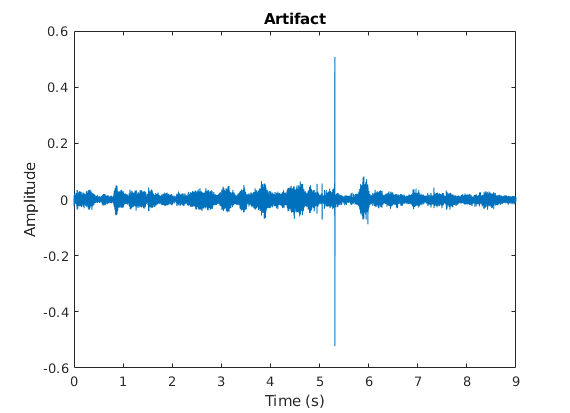
\includegraphics[scale = 0.45]{./arti.png}
    \caption{Artifact Class signal}
    \label{fig:arti}
\end{figure}{}

From figure \ref{fig:arti}, it can be seen that there is no sense of normal periodicity within the signal.







\end{document}

" vim: ts=4
" vim: tw=78
" vim: autoindent
" vim: shiftwidth=4
